\documentclass[a4paper, 11pt, normalem]{report}

\usepackage{../../../LaTeX-Templates/Notes}
\usepackage{subfiles}

\title{Condensed Matter Physics \vspace{-20pt}}
\author{Prof Hatton and Dr Mendis}
\date{\vspace{-15pt}Epiphany Term 2019}
\rhead{\hyperlink{page.1}{Contents}}

\begin{document}

\maketitle
\tableofcontents

\part{}
%Hatton
\chapter{Free and Nearly Free Electrons}
\begin{wrapfigure}{r}{0.4\textwidth}
    \centering
    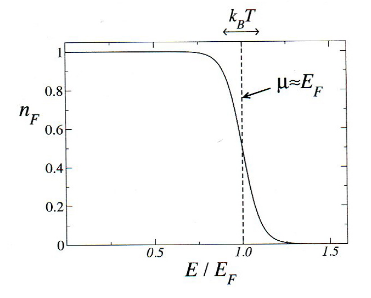
\includegraphics[width=0.4\textwidth]{fd.png}
\end{wrapfigure}
Given that electrons are fermions, we will use the Fermi-Dirac distribution. 
\begin{equation}
    n_F = \frac{1}{(e^{E-\mu/k_BT)}+1}
\end{equation}
We will consider electron waves in a box $V=L^3$ with periodic boundary conditions. 
The plane wavefunctions of the electron waves are of the form $e^{ik\cdot r}$ with wavevectors $(\frac{2\pi}{L})(n_1,n_2,n_3)$.
The plane waves have energies,
\begin{equation}
    E(k) = \frac{\hbar^2|k|^2}{2m}
\end{equation}
where $m$ is the electron mass. 

\begin{wrapfigure}{r}{0.4\textwidth}
    \centering
    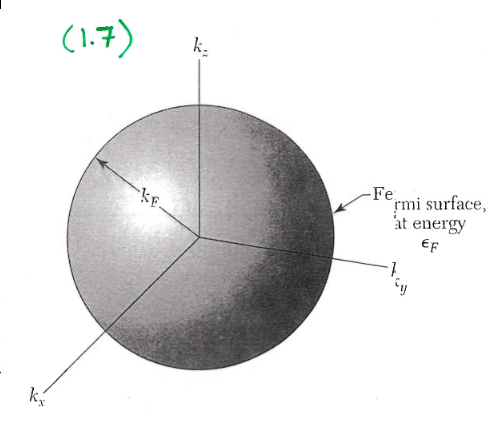
\includegraphics[width=0.4\textwidth]{fermisph.png}
\end{wrapfigure}
Thus the total number of electrons in the system is 
\begin{equation}
    N = 2\sum_k n_f\left(\frac{\e(k) - \mu}{k_BT}\right) = 2\frac{V}{(2\pi)^3}\int dk n_F\left(\frac{\e(k) - \mu}{k_BT}\right)
\end{equation}
where the prefactor of 2 accounts for the two possible spin states for each wavevector. 
We can define the Fermi energy as equal to $\mu$ at $T=0$.
\begin{equation}
    E_F = \frac{\hbar^2k_F^2}{2m}
\end{equation}
\begin{itemize}
    \item Fermi temperature, $T_F = \frac{E_F}{k_B}$
    \item Fermi momentum, $p_F = \hbar k_F$
    \item Fermi velocity, $v_F = \hbar k_F/m$
\end{itemize}
\begin{equation}
    N = 2\frac{V}{(2\pi)^3}\left(\frac{4}{3}\pi k_F^3\right)
\end{equation}
This plots a Fermi sphere.

At $T=0$, the electrons fill a sphere (the Fermi sphere) of radius $k_F$.
The surface of the sphere is known as the Fermi surface and delineates filled states from unfilled states. 
The density of free electrons,
\begin{align}
    n &= \frac{N}{V} \\
    \implies k_F &= (3\pi^2n)^{1/3} \\
    \implies E_F &= \frac{\hbar^2(3\pi^2n)^{2/3}}{2m}
\end{align}

Many problems with the Sommerfeld free electron theory, e.g. The Hall Effect
\begin{equation} 
    R_H = \frac{-1}{n_e}
\end{equation}
Sometimes too high (e.g. Bi), sometimes too low (e.g. Al).

The heat capacity of metals
\begin{equation}
    C = \gamma T + \alpha T^3
\end{equation}
does not have a zero intercept.
Values of $\gamma_{exp}$ vary from $0.2\gamma_{theory}$ to $50\gamma_{theory}$, suggesting that $m$, the electron mass, is a variable. 
\begin{figure}[H]
    \centering
    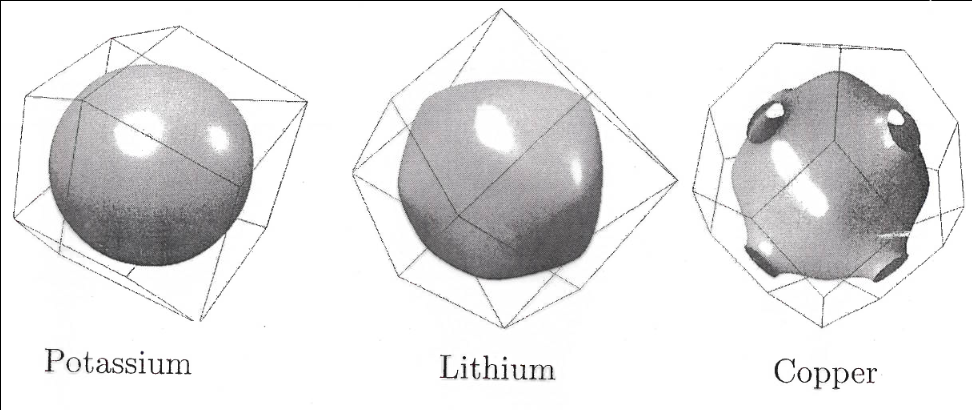
\includegraphics[scale=0.4]{spheres.png}
    \caption{Whilst some Fermi spheres are spherical (e.g. Potassium), others (e.g. Copper) are not}
\end{figure}

\chapter{}
Consider a one-dimensional chain of atoms with spacing $a$ between them. 
The figure below shows the low energy portion of the band structure for (a) free electrons, and (b) nearly-free electrons with an energy gap at $k = \pm \frac{\pi}{a}$.
\begin{figure}[H]
    \centering
    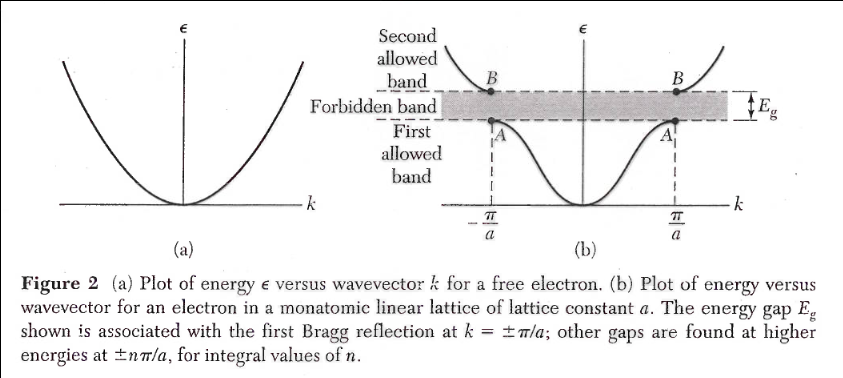
\includegraphics[scale=0.5]{brill.png}
\end{figure}
The Bragg condition $(k+G)^2 = k^2$ for diffraction of a wave of wavevector $k$ then becomes 
\begin{equation}
    l = \pm \frac{G}{2} = \pm \frac{n\pi}{a}
\end{equation}
where $G = \frac{2n\pi}{a}$ is a reciprocal lattice vector and $n$ is an integer.
The first reflections and the first energy gap occur at $k = \pm \frac{\pi}{a}$.
The region in k-space between $-\frac{\pi}{a}$ and $+\frac{\pi}{a}$ is the first Brillouin zone of the lattice.
Higher energy gaps occur for other values of $n$.

The wavefunctions at $\pm \frac{\pi}{a}$ of the form $\exp{(\pm i\pi x/a)}$ are not the plane travelling waves we might expect.
At these special values of $k$, the wavefunctions are made up of equal parts of waves traveling to the right, and waves traveling to the left. 
At the Brillouin zone boundaries, the wave is reflected back. 

The time-independent result is a standing wave.
We can form 2 different standing waves,
\begin{align}
    \Psi(+) &= \exp{\left(\frac{i\pi x}{a}\right)}  + \exp\left(\frac{-\pi x}{a}\right) = 2\cos\left(\frac{\pi x}{a}\right) \\
    \Psi(-) &= \exp\left(\frac{i\pi x}{a}\right) - \exp\left(\frac{-i\pi x}{a}\right) = 2i\sin\left(\frac{\pi x}{a}\right) 
\end{align}
The two standing waves $\Psi(+)$ and $\Psi(-)$ pile up electorn density in different regions, and have different energies. 
The probability density $P$ is $\Psi^*\Psi = |\Psi|^2$.
For a traveling plane wave, $P = \exp(-ikx)\exp(ikx) = 1$.
But $\Psi(+)$ has a density, 
\begin{equation}
    P(+) = |\Psi(x)|^2 \propto \cos^2\left(\frac{\pi x}{a}\right)
\end{equation}
This concentrates electron density at the postive ions. 
\begin{figure}[H]
    \centering
    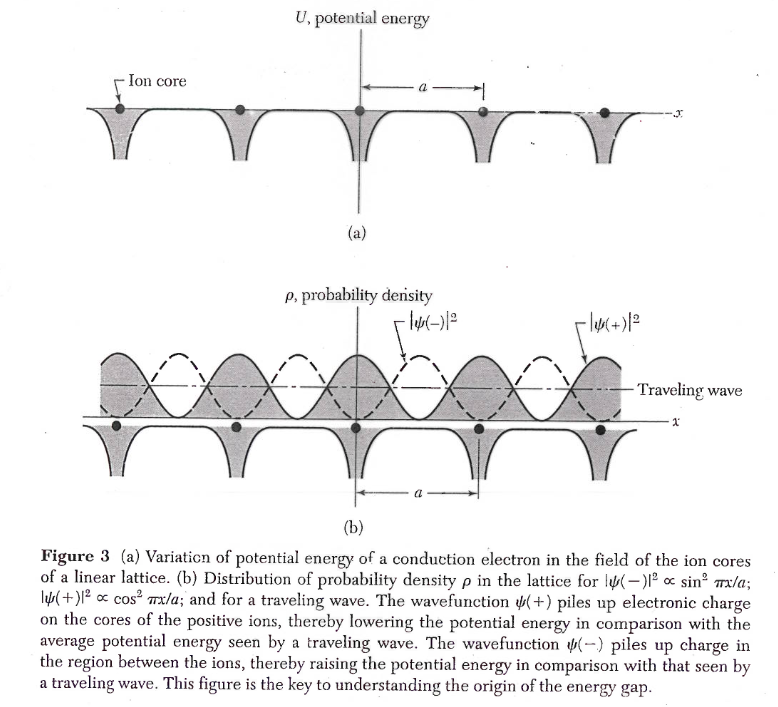
\includegraphics[scale=0.5]{l2f3.png}
\end{figure}
The standing wave $\Psi_+$ concentrates the electron density at the ion cores where the potential energy is at its lowest. 
This cause a lowering of the energy of $\Psi_+$.
For the other standing wave, $\Psi_-$, the probability density is
\begin{equation}
    P(-) = |\Psi|^2 \propto \sin^2\left(\frac{\pi x}{a}\right)
\end{equation}
which concentrate $e^-$ density between the positive ion cores - Bad News. 

Thus at the Brillouin zone boundary, 
\begin{equation}
    k = \big|\frac{\pi}{a}\big|
\end{equation}
The two standing waves exist with the same wavevector but different energies.

The wavefunctions at the Brillouin zone boundary $k=\frac{\pi}{a}$ are $\sqrt{2}\cos(\frac{\pi x}{a})$ and $\sqrt{2}\sin(\frac{\pi x}{a})$, normalised over unit length. 
If the PE of an electron in the one dimensional chain at point $x$ is
\begin{equation}
    U(x) = U\cos\left(\frac{2\pi x}{a}\right)
\end{equation}
Then the first-order energy different between the two standing waves is
\begin{align}
    E_g &= \int_0^1 dx ~ U(x) \left[|\Psi_+|^2 - |\Psi_-|^2\right] \\
        &= 2\int dx ~ U(x) \cos\left(\frac{2\pi x}{a}\right)\left(\cos^2\left(\frac{\pi x}{a}\right) - \sin^2\left(\frac{\pi x}{a}\right) \right) \\
        &= U
\end{align}
We see that the energy gap $E_g$ is equal to the Fourier component of the crystal potential.

\section{Model 2}
We will again start with plane electron waves perturbed by a periodic potential and use second-order perturbation theory from QM.

We start with completely free electrons whoes Hamiltonian is 
\begin{equation}
    \Ham_0 = \frac{p^2}{2m}
\end{equation}
The plane waves $|k\rangle$ have eigenenergies
\begin{equation}
    \e_0(k) = \frac{\hbar^2|k|^2}{2m}
\end{equation}
We consider a weak potential perturbation, 
\begin{equation}
    \Ham = \Ham_0 + V(r)
\end{equation}
with V periodic, $V(r) = V(r+R)$, where $R$ is any lattice vector.

The matrix elements of this potential are the Fourier components
\begin{equation}
    \langle k'|V|k\rangle = \frac{1}{L^3} \int dr~ e^{i(k-k')\cdot r} V(r) \equiv V_{k-k'}
\end{equation}
which is zero unless $k-k'$ is a reciprocal lattice vector. 

So any plane wave state $k$ can only scatter into another $k'$ if the two plane waves are separated by a reciprocal lattice vector.
Now, we apply the rules of perturbation theory. 
At first order, 
\begin{equation} 
    \e(k) = \e_0(k) + \langle k|V|k\rangle = \e_0(k) + V
\end{equation}
Just an energy shift. Assume $V_0 = 0$.

At second order, 
\begin{equation}
    \e(k) = \e_0(k) + \sum_{k'=k+G}' \frac{|\langle k'|V|k\rangle|^2}{\e_0(k) - \e_0(k')}
\end{equation}
where ' means the sum is restricted to have $G\neq 0$.
Be careful - for some $k'$ then $\e_0(k)$ may be very close to $\e_0(k')$. 
Then the sum will diverge. 
Therefore, we need degenerate perturbation theory. 
To see when this degenerate situation occurs, look for solutions of
\begin{align}
    \e_0(k) &= \e_0(k') \\
    k' = k+G
\end{align}
Let us return to our 1D case. 
Since $\e(k) \approx k^2$ then the only possible solution is 
\begin{equation}
    k' = -k
\end{equation}
This means the two equations are only satisfied for 
\begin{equation} 
    k' = -k = \frac{n\pi}{a} 
\end{equation}
Precisely on the Brillouin zone boundaries. 
This is generally true, in 1D, 2D, 3D, etc. 
So, when we are very near a zone boundary, our second order is divergent and we need degenerate perturbation theory. 
In this approach we diagonalise the Hamiltonian within the degenerate space first.

\section{Degenerate Perturbation Theory}
If our two plane wave states $|k\rangle$ and $|k'\rangle = |k+G\rangle$ are of approximate equal energy, then we diagonalise matrix elements first. 
We have
\begin{align}
    \langle k|H|k\rangle &= \e_0(k) \\
    \langle k'|H|k'\rangle &= \e_0(k') = \e_0(k+G) \\
    \langle k|H|k'\rangle &= V_{k-k'} = V^*_G \\
    \langle k'|H|k\rangle &= V_{k'-k} = V_G
\end{align}
Within this two-dimensional space, we can write any wavefunction as
\begin{equation}
    |\psi\rangle = \alpha|k\rangle + \beta|k'\rangle = \alpha|k\rangle + \beta|k+G\rangle
\end{equation}
Using the variational principle to minimise the energy is like solving the effective Schrodinger equation,
\begin{equation}
    \begin{pmatrix}
        \e_0(k) & V_G^* \\
        V_G & \e_0(k+G) 
    \end{pmatrix}
    \begin{pmatrix}
        \alpha \\
        \beta
    \end{pmatrix} = E
    \begin{pmatrix}
        \alpha \\
        \beta
    \end{pmatrix}.
\end{equation}
The characteristic equation determining $E$ is then
\begin{equation}
    [\e_0(k) - E][\e_0(k+G) - E] - |V_G|^2 = 0
\end{equation}

\section{Life at the Brillouin Zone Boundary}
At the Brillouin zone boundary, $k' = k+G$ and hence
\begin{equation}
    \e_0(k) = \e_0(k+G).
\end{equation}
Then the characteristic equation simplifies to
\begin{equation}
    [\e_0(k) - E]^2 = |V_G|^2
\end{equation}
or equivalently,
\begin{equation}
    E_{\pm} = \e_0(k) \pm |V_G|.
\end{equation}
Thus a gap opens up at the zone boundary. 
In the free electron theory, $k$ and $k'$ both had an energy, $\e_0(k)$. 
When we add a periodic potential, $V_G$, the two eigenstates form two linear combinations whose energies differ by $\pm |V_G|$.
Just like in Model 1.

\section{Nearly-free electron WFs in 1D}
To understand what the wavefunctions look like, let us retreat to our 1D chain of atoms. 
Let us assume we have a potential, 
\begin{equation}
    V(x) = \tilde{V}\cos\left(\frac{2\pi x}{a}\right),~ \tilde{V} > 0
\end{equation}
The Brillouin zone boundaries are at $k = \frac{\pi}{a}$ and $k' = -k = -\frac{\pi}{a}$ so that $k' -k = G = -\frac{2\pi}{a}$ and $\e_0(k) = \e_0(k')$.
Examining the effective Schrodinger equation, we discover that the solutions (when $\e_0(k) = \e_0(k')$) are given by $\alpha = \pm \beta$, which gives eigenstates, 
\begin{equation}
    |\psi_{\pm}| = \frac{1}{\sqrt{2}}(|k\rangle \pm |k'\rangle),
\end{equation}
corresponding to the eigenenergies, $E_\pm$.
We can write the real (direct) space version of these $|k\rangle$ wavefunctions as 
\begin{align}
    |k\rangle &\to e^{ikx} = e^{ik\pi/a} \\
    |k\rangle &\to e^{-ik'x} = e^{-ik'\pi/a}
\end{align}
Thus, the two eigenstates are given by
\begin{align}
    \psi_+ &\approx e^{ix\pi/a} + e^{-ix\pi/a} \\
           &\propto \cos\left(\frac{x\pi}{a}\right) \\
    \psi_- &\approx e^{ix\pi/a} - e^{-ix\pi/a} \\
           &\propto sin\left(\frac{x\pi}{a}\right)
\end{align}
And the densities $|\psi_\pm|^2$ associated with these two wavefunctions are shown - just like in Model 1.











\part{}
%Mendis

\end{document}
